\section{Volumes com cálculo complicado}
\label{sec:volumes-dificeis}

O uso de integrais duplas para o cálculo de volumes (ver
equação~\ref{eq:volumeexato}) é aplicável em diversas situações e
em diferentes funções. Entretanto, existem funções nas quais o cálculo do
volume é difícil. Considere, por exemplo, o cálculo do volume do
sólido limitado abaixo pelo plano $z = 0$ e acima pelo parabolóide $z
= 1 - x^2 - y^2$ (figura~\ref{fig:voldif}):

\begin{figure}[H]
  \begin{center}
    \caption{Como calcular esse volume?}
    \label{fig:voldif}
    \fbox{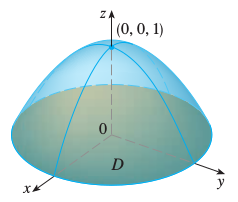
\includegraphics[scale=0.7]{imagens/int07.png}}\\
    \footnotesize{James Stewart: \emph{Cálculo} (8ª ed.,\ vol.\ 2,
      pg.\ 906)}
  \end{center}
\end{figure}

Note que a base não é mais um retângulo, é um disco $D$. Se tentarmos
calcular o volume através da utilização direta da
equação~\ref{eq:volumeexato}, chegaremos em uma expressão muito
difícil de resolver:

\begin{equation*}
    \begin{split}
      V &= \iint\displaylimits_D (1-x^2-y^2) \diff A\\
        &= \int_{-1}^1 \int_{-\sqrt{1-x^2}}^{\sqrt{1-x^2}}(1-x^2-y^2)
      \diff y \diff x
    \end{split}
\end{equation*}

E por que é difícil calcular o volume de funções parecidas com a
ilustrada na figura~\ref{fig:voldif}? Pois a ``base'' do sólido não é
mais um retângulo, é um disco, e, já que estamos utilizando o sistema
de \emph{coordenadas retangulares}, não é possível descrever o disco $D$ formado
por $x$ e $y$ por uma única função (ver figura~\ref{fig:voldif2}):

\begin{figure}[H]
  \begin{center}
    \caption{O disco $D$ não pode ser descrito por uma única função}
    \label{fig:voldif2}
    \fbox{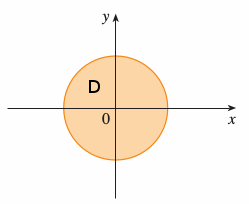
\includegraphics[scale=0.7]{imagens/int08.png}}\\
    \footnotesize{James Stewart: \emph{Cálculo} (8ª ed.,\ vol.\ 2,
      pg.\ 904)}
  \end{center}
\end{figure}

Para poder calcular esses volumes difíceis temos que mudar nosso ponto
de vista\footnote{Uma animação interessante que mostra como mudar o
  ponto de vista muda nosso entendimento sobre uma função pode ser
  vista em \url{http://www.youtube.com/watch?v=Dmc3mQ87GiQ}.}:
precisamos sair do sistema de coordenadas retangulares e
utilizar o sistema de \emph{coordenadas polares}.

A próxima seção explicará o que é o sistema de coordenadas polares
para, a partir desse conhecimento, demonstrar como o cálculo integral
pode ser feito utilizando-se esse referencial.
